%%%%%%%%%%%%%%%%%%%%%%%%%%%%%%%%%%%%%%%%%%%%%%%%%%%%%%%%%%%%%%%%%%
\section{Smart Grids}
\label{sec:smartgrids}


En las últimas décadas, se ha observado una transformación integral del modelo asociado a la red eléctrica convencional. El aumento de la energía demandada por los usuarios finales y los requisitos cada vez mayores de la industria ha tenido como consecuencia que algunos países hayan intentado diseñar redes eléctricas agrupadas en un conjunto de grandes redes nacionales. De este modo, todas las fuentes energéticas disponibles pueden estar conectadas para ser gestionadas conjuntamente en función de la demanda recibida, además de conseguir una coordinación a alto nivel. \cite{smartgrid_overview}

\vspace{3mm}

No obstante, una red eléctrica no se puede definir como una entidad única e independiente, pues se trata de una agregación de redes, compañías energéticas y operadores que trabajan en distintos niveles de comunicación. Es por ello, que la idea de desarrollar una gran red nacional encuentra cierto equilibrio energético, pero no llega a los altos porcentajes de eficiencia que pueden proveer las redes inteligentes energéticas o de otra forma, las \textit{smart grids} (\gls{sg}). 

\vspace{3mm}

Una \textit{smart grid} \cite{iotfutura} \cite{repsol} se define como una red inteligente con la capacidad de distribuir los suministros de energía de forma optimizada a los usuarios, basándose en la información que recoge de los mismos. Es por ello que supone una actualización digital de las redes de distribución y transmisión a larga distancia para incorporar sistemas de monitorización y control a tiempo real.

\vspace{3mm}

En otros términos, su base se asienta en el diseño de sistemas inteligentes coordinados capaces de obtener tanto la información respectiva a la demanda o requisitos energéticos de cada zona como la de la disponibilidad de recursos a partir de las diferentes fuentes de producción existentes. Todo ello conduce al desarrollo de un plan estratégico de distribución energética para poder conectar a todas las entidades participantes en la red entre sí.

\vspace{3mm}

Cabe destacar que una de las principales características diferenciadoras de las \gls{sg} respecto a las redes energéticas convencionales es que se fundamentan en una comunicación bidireccional. Este factor determinante se puede apreciar en la Figura \ref{fig:bidireccional} y se traduce en una producción y una distribución dinámica y personalizada hacia cada usuario de la red. 

\vspace{3mm}

\begin{figure}[h]
  \centering
  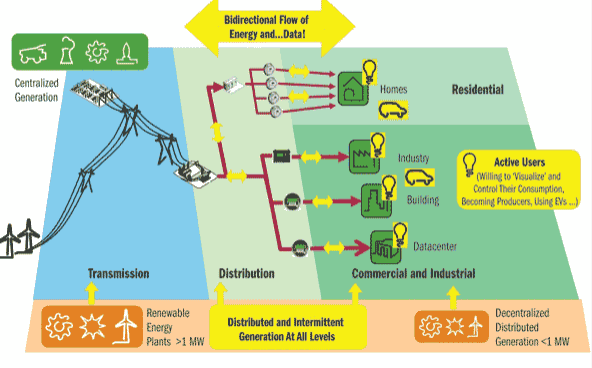
\includegraphics[width=0.9\textwidth]{img/teoria/sg.png}
  \caption{Flujo bidireccional de datos y energía en una \textit{smart grid} \cite{sins}}
  \label{fig:bidireccional}
\end{figure}

\vspace{3mm}

Es decir, en una red tradicional al ser unidireccional, se provee energía desde el distribuidor hacia el consumidor sin llevar a cabo ningún análisis estadístico sobre el consumo que se está produciendo en las líneas finales en un determinado instante temporal. En cambio, en el contexto de las \gls{sg}s, se pone el foco en las acciones de los usuarios y en la consecuente asignación de patrones de consumo eléctrico que permita predecir el comportamiento futuro de los mismos. \cite{convencional}

\vspace{3mm}

Teniendo en cuenta esto, se puede decir que los propios usuarios son el gran pilar sobre el que se cimienta la red. En comparación a la red eléctrica tradicional, toman un papel mucho más activo monitorizando continuamente su comportamiento eléctrico y recopilando información para trasladarla al resto de la red. Esto tiene como ventaja una gran reducción de los costes derivados de la distribución y transmisión en el sistema, ya que se evita proporcionar más cantidad de energía de la requerida por las líneas finales. \cite{iotfutura}

\vspace{3mm}

No obstante, como se expondrá más adelante en la Sección \ref{sec:consumo}, este proceso de clasificación de usuarios requerirá del análisis de grandes volúmenes de datos adquiridos a tiempo real, por lo que se aumentará la complejidad del sistema a costa de alcanzar la eficiencia.



\vspace{3mm}


\cite{impact}


% así como para abrir nuevos mercados para la producción de energía alternativa.
En este contexto se introduce el término de prosumidor.



%sin interferencia humana. 








%According to the IEEE smart grid initiative [1], “the smart grid is a revolutionary undertaking—entailing new communications-and-control capabilities, energy sources, generation models and adherence to cross-jurisdictional regulatory structures”.
%La implementación de Smart Grid es imperativa, no sólo en Estados Unidos sino en todo el mundo. Pero la red inteligente es una empresa revolucionaria que implica nuevas capacidades de comunicaciones y control, fuentes de energía, modelos de generación y adhesión a estructuras regulatorias interjurisdiccionales. Una implementación exitosa exigirá colaboración, integración e interoperabilidad objetivas entre una fenomenal variedad de disciplinas, incluidos sistemas de control computacional y de comunicaciones para generación, transmisión, distribución, clientes, operaciones, mercados y proveedores de servicios.


%https://smartgrid.ieee.org/about-ieee-smart-grid

%ver tablasecciones.pdf






%%ventajas  


\cite{repsol} 

% Mayor flexibilidad
% La automatización de los procesos y la aplicación de sistemas inteligentes permite responder rápidamente a cualquier imprevisto o avería y dar una respuesta inmediata, incluso en remoto.

% Aumento de la seguridad
% El circuito interconectado de una smart grid proporciona un suministro eléctrico todavía más fiable, eficiente, seguro y sostenible, lo que supone una mejora en la calidad del servicio.

% Respuesta a la demanda y ahorro
% Permiten que los usuarios conecten sus dispositivos electrónicos en las franjas en las que las tarifas son más bajas. Lo que se traduce en un ahorro directo en la factura de la luz. 

% Gestión de la carga
% Gracias a las smart grid los usuarios pueden saber en tiempo real la electricidad y la tarifa a la que están consumiendo energía. Esto permite gestionar y reducir el uso de la misma, lo que evitaría, por ejemplo, un caso de carga elevada.

% Descentralización de la producción
% Los usuarios no solo son consumidores, sino que también pueden generar energía. A través de las smart grid el excedente de energía se puede almacenar o trasladar a la red eléctrica general para que otros usuarios puedan consumirla. 


%Las smart grid son un concepto estratégico clave en la transición energética, ya que suponen un gran paso hacia un mundo descarbonizado. Mediante la digitalización de las redes eléctricas inteligentes se puede conseguir un sistema más eficiente, sostenible, con bajas pérdidas y con altos niveles de calidad en el suministro. Con la implementación de este circuito inteligente no solo se conseguiría una mayor eficiencia energética y ahorro, sino que también tendría múltiples beneficios medioambientales, económicos y sociales.

% Beneficios ambientales

% La eficiencia energética que se pueden conseguir con las smart grid también tiene beneficios directos sobre el medio ambiente, como por ejemplo: 

% Permiten el desarrollo de ciudades sostenibles.
% Pueden integrarse en el sistema de fuentes renovables.
% Facilitan la movilidad eléctrica, proporcionando puntos de carga para vehículos eléctricos.
% Reducen las emisiones globales de CO2.
% Contribuye a la descarbonización de la generación eléctrica. 



% Beneficios económicos

% Un sistema de red eléctrica eficiente tiene beneficios económicos, entre los que destacan:

% Accesibilidad de la información. Gracias a la recopilación de estos datos, la compañía eléctrica y los consumidores pueden reducir los costes.
% Permite minimizar el coste de las operaciones. Y, en consecuencia, el coste para el consumidor final.
% Facilita el almacenamiento de electricidad y mejora la eficacia en la distribución de los flujos de energía por lo que no hay desperdicios.
% Mayor control de reparaciones localizando el corte energético de manera inmediata.
% Existen menos picos de demanda, lo que se traduce en una bajada de los precios. 



% Beneficios sociales

% La implementación de las redes eléctricas smart grid repercute directamente en la sociedad: 

% Permiten una respuesta inmediata, asegurando un sistema energético eficiente.
% Aumentan el nivel de seguridad, fiabilidad y de calidad del servicio.
% Posibilitan conocer el consumo y tarifa aplicada en tiempo real.
% El usuario es parte activa y fundamental del proceso. Puede gestionar el consumo de energía, verter sus excedentes a la red de energía eléctrica o almacenarlo para utilizarlo en otro momento.
% En caso de interrumpir el servicio, el restablecimiento es más rápido.


\cite{smartgrid_overview}

%Algunos de los beneficios de una red eléctrica modernizada incluyen la capacidad para reducir el consumo de energía en el lado del consumidor durante las horas pico, llamado gestión de la demanda; permitir la conexión a la red de generación distribuida de energía (con matrices fotovoltaicas, pequeños aerogeneradores, microhidroeléctricas o incluso generadores combinados de calor y energía en edificios); incorporar el almacenamiento de energía en la red para equilibrar la carga de generación distribuida; y eliminar fallas como fallas en cascada de la red eléctrica. Se espera que la mayor eficiencia y confiabilidad de la red inteligente ahorren dinero a los consumidores y ayuden a reducir las emisiones de CO2. Dado el creciente enfoque gubernamental en la seguridad energética, invertir en la red inteligente podría utilizarse para reducir la dependencia de fuentes de energía no domésticas y hacer que la red sea más resistente a ataques militares o terroristas, ya sea por medios físicos o digitales.





















%%%%ESPAÑA HABLAR AQUI DE RED DE ESPAÑA

%http://www.geni.org/globalenergy/library/national_energy_grid/spain/index.shtml

%Spain has the fifth largest electricity market in Europe (behind Germany, France, the United Kingdom, and Italy), and it is growing quickly. Electricity demand for 2001 was estimated to be 210.4 billion kilowatthours (bkwh), a 5% increase over 2000. It is estimated that Spain's electricity demand will increase 30% by 2010.

%To meet Spain's increased demand for electricity, domestic utility companies have invested in generation capacity and distribution. Red Electrica de España (REE), for instance, invested heavily in the network in 2001, dedicating 78.4 million euros to expanding the electricity network. REE also announced plans in October 2001 to invest between 60.2 and 72.2 million euros to improve the electricity connection with France. Spain's three largest electricity groups - Endesa, Iberdrola, and Union Fenosa - have dedicated 34 billion euros of investments from August 2001 to 2005, with much of that in Latin America and other European countries, but nevertheless including 8 billion euros for new generating plants in Spain.

%Endesa is in the process of building a natural-gas-fired, 400 MW, combined-cycle generating turbine (CCGT) plant in Huelva in addition to two other gas-fired 400-MW CCGTs the company already has under construction in Barcelona and Tarragona. Endesa recently completed the construction of a plant with 8,000 MW in Cadiz. Union Fenosa plans to add 5,000 MW of new capacity by 2005, mostly in Spain, of which 2,800 MW would be natural-gas-fired. Piemsa, an affiliate of Petronor, is planning to construct an 800-MW integrated gasification combined-cycle(IGCC) complex at a refinery near Bilbao that will make use of heavy refinery stocks. The plant will be one of the largest and most advanced of its kind in the world.

\vspace{3mm}

\begin{figure}[h]
  \centering
  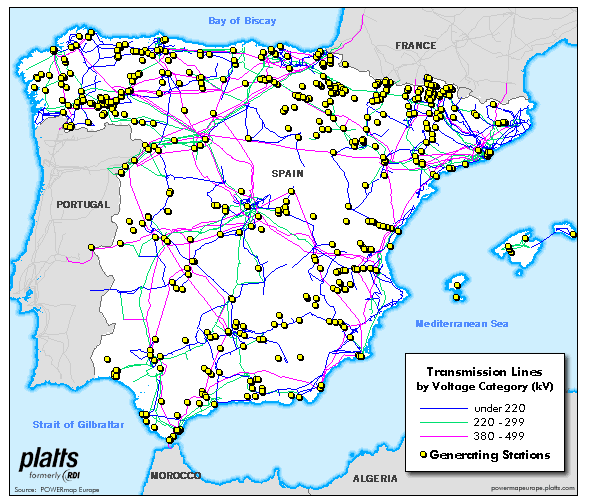
\includegraphics[width=0.8\textwidth]{img/teoria/spain.png}
  \caption{Red nacional de transmisión energética \cite{spain}}
  \label{fig:spain}
\end{figure}

\vspace{3mm}

%%%%%%%%%%%%%%%%%%%%%%%%%%%%%%%%%%%%%%%%%%%%%%%%%%%%%%%%%%%%%%%%%%
\subsection{Internet of Energy}
\cite{ioe}




%%%%%%%%%%%%%%%%%%%%%%%%%%%%%%%%%%%%%%%%%%%%%%%%%%%%%%%%%%%%%%%%%%
\subsection{Estructura de una Smart Grid}

Una \gls{sg} está constituida por múltiples elementos diferentes como se puede visualizar en la Figura \ref{fig:estructura_sg}. Cada uno de ellos está dedicado a uno de los procesos principales, que se pueden dividir en generación, distribución y consumo. \cite{smartgrid_overview}

\vspace{3mm}

\begin{figure}[h]
  \centering
  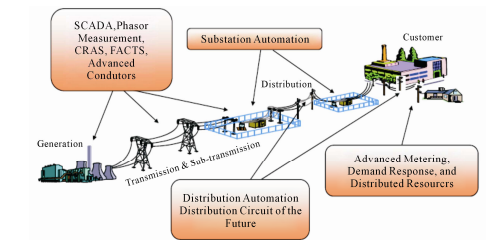
\includegraphics[width=1\textwidth]{img/teoria/estructura_sg.png}
  \caption{Estructura de componentes de una \gls{sg} \cite{smartgrid_overview}}
  \label{fig:estructura_sg}
\end{figure}

\subsubsection{Generación y distribución}

\vspace{3mm}

Dentro del contexto de la generación de energía destacan los sistemas de control y adquisición de datos (del inglés \gls{scada}) \cite{scada}. Estos pueden ser instalados en generadores, como son paneles solares fotovoltaicos o turbinas eólicas, consiguiendo una monitorización remota de los mismos. Mediante la información recopilada a tiempo real permiten conocer los niveles de generación y establecer una predicción de la disponibilidad energética que habrá en el sistema o en un área determinada del mismo.

\vspace{3mm}

Otro dispositivo importante en el campo de la generación y de la distribución energética es la Unidad de Medición de Fasores (del inglés \gls{pmu}). Se emplea para medir con una alta precisión los fasores de tensión y corriente en la red eléctrica, proporcionando información relevante sobre las magnitudes y fases de las ondas sinusoidales. Debe contar con una alta tasa de muestreo para capturar eventos transitorios o cambios rápidos en la red y, en consecuencia, tener la capacidad de identificar o detectar a tiempo real posibles anomalías que se puedan dar en la distribución. Es por ello que, el \gls{pmu} se trata de un componente imprescindible para comprobar y garantizar la estabilidad de la \gls{sg}. %BIB

\vspace{3mm}

La confiabilidad y la seguridad de la red también reside en los Sistemas de Transmisión de Corriente Alterna Flexibles (del inglés \gls{facts}) \cite{facts} \cite{facts3}. Estos vienen dados por la necesidad de superar las limitaciones técnicas introducidas por las redes eléctricas, como son las térmicas o las respectivas al voltaje. En otros términos, incrementan la potencia transmitida y aportan flexibilidad al permitir modificar de forma dinámica los parámetros eléctricos ante cambios en la configuración de la red. 

\vspace{3mm}

Los \gls{facts} incluyen todos los elementos electrónicos basados en tecnología de alta potencia y que son empleados dentro de una \gls{sg} para la transferencia de energía de CA y el control de la potencia reactiva. También, realizan tareas de reducción de impedancia en las líneas de transmisión y de optimización del factor de potencia y pueden actuar tanto a nivel individual como de forma coordinada con otros controladores.

\vspace{3mm}

La primera generación de \gls{facts} emplea interruptores controlados por tiristores, mientras que la segunda tiene como base convertidores estáticos de conmutación. En la Tabla \ref{tab:facts} se visualizan las tecnologías \gls{facts} más relevantes. \cite{facts2} \cite{facts3}

\vspace{3mm}

\begin{table}[!h]
    \centering
    \resizebox{\textwidth}{!}{
    \begin{tabular}{| c | c | m{6cm} |}
    \hline
    \rowcolor[HTML]{EFEFEF}
    Generación & Tipo & \multicolumn{1}{c|}{Descripción} \\ \hline
    \multirow{2}{*}{1º} 

    & \gls{tcsc} & Controla el flujo de potencia tanto reactiva como activa por la línea de transmisión mediante el ajuste de impedancia en serie y amortigua las oscilaciones.
    
    \\ \cline{2-3}

    & \gls{svc} & Absorbe o suministra potencia reactiva según las necesidades de una línea de transmisión a través de la variación de la susceptancia en paralelo. Ayuda a mantener el voltaje estable en la red y proveen un aumento de la capacidad de transferencia de energía.

    \\ \hline
    \multirow{4}{*}{2º} 
    
    & \gls{statcom} & Compensa la potencia reactiva al igual que el \gls{svc}, pero en este caso empleando electrónica de potencia para proporcionar una respuesta más rápida.

    \\ \cline{2-3} 

    & \gls{upfc} & Combina las funciones de un \gls{tcsc} y un \gls{svc}, teniendo la capacidad de controlar en una línea de transmisión tanto la impedancia en serie como la susceptancia en paralelo.

    \\ \cline{2-3} 

    & \gls{sssc} & Modifica dinámicamente la impedancia y es capaz de controlar la fase y la amplitud de la tensión en la línea.

    \\ \cline{2-3} 

    & \gls{ipfc} & Conecta varias líneas de transmisión en paralelo. No obstante, modula la impedancia y la fase de la tensión de cada línea de transmisión de forma independiente, lo que permite operar sobre el flujo de potencia de una forma controlada. Mejora la capacidad de transmisión y reduce las pérdidas energéticas. 
    
    \\ \hline
    \end{tabular}
    }
    \caption{Tecnologías FACTS de 1ª y 2ª generación}
    \label{tab:facts}
\end{table}

\vspace{3mm}

Poniendo el enfoque en la garantía de estabilidad de una \gls{sg}, uno de los sistemas más importantes de los expuestos en la Tabla \ref{tab:facts} es el \gls{svc} \cite{facts}. Los compensadores estáticos son capaces de detectar grandes caídas de tensión resultantes a la producción de un cortocircuito o a la pérdida de líneas de transisión en un área de la red. Esto es importante, ya que una detección rápida de una avería permite restaurar en un corto período de tiempo la tensión del área afectada sin que el problema escale a otras partes de la red. 

\vspace{3mm}

En otros términos, aísla este área del resto de la red eléctrica. Además, el \gls{svc} asegura que el proceso de restauración se produzca paulatinamente para que los efectos producidos por el cortocircuito sean prácticamente imperceptibles en los puntos de carga del área afectada. En la Figura \ref{fig:svc} se puede apreciar un ejemplo de instalación de un \gls{svc} en el municipio noruego Sylling y se encuentra conectada a un sistema de 420 kV.

\vspace{3mm}

\begin{figure}[h]
  \centering
  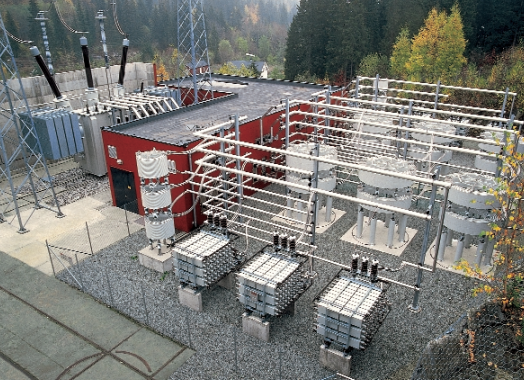
\includegraphics[width=0.7\textwidth]{img/teoria/svc.png}
  \caption{Instalación de un \gls{svc} en Sylling (Noruega) \cite{facts}}
  \label{fig:svc}
\end{figure}

\subsubsection{Consumo}
\label{sec:consumo}

Entrando en detalle en las ubicaciones finales del sistema y por tanto, en el proceso de consumo, es imprescindible conocer la cantidad de energía demandada por los clientes que pertenecen a una \gls{sg}. La instalación de sensores o medidores inteligentes (del ingles \textit{smart meters}) en las viviendas posibilitan el registro constante de datos respectivos al consumo de energía, niveles de voltaje, corriente y factor de potencia. Estos son almacenados, analizados y procesados por las distribuidoras de energía para obtener a partir de los mismos la información necesaria sobre el comportamiento de los usuarios. \cite{stab}

\vspace{3mm}

%cite -> Renewable energy management in smart grids by using big data analyticsand machine learning
% Managing these grids requires efficient real-time data processing
% and analysis of the massive amount of data captured by monitors,
% sensors, meters, cameras and computers to both improve the efficiency
% and to avoid delays and system shutdowns (Chen et al., 2014). This
% data is used for many different applications: real-time vulnerability
% assessment, demand management, predictive analytics, theft detection,
% energy trading, economic dispatch, etc. (Asad & Chaudhry, 2017). It
% is considerably difficult to manage these large and diverse datasets
% through using traditional database management tools; this type of
% data, namely ‘Big data’ requires advanced management approaches.
% Big data is a computer science technology that can be applied to data
% from different and uncorrelated sources, which make it hard to use
% traditional data analysis tools to process this data. It is characterized
% by its four main components: Variety, Velocity, Volume and Veracity,
% namely ‘the 4Vs’ (Wang et al., 2019). The ‘Varity’ component refers
% the different sources and types of data to be processed. The ‘Velocity’
% component refers to the need for fast and synchronized processing and
% analysis of data. The ‘Volume’ component refers to the ability to handle
% large and growing amount of data (Sagiroglu & Sinanc, 2013). Finally,
% the ‘Veracity’ component is concerned with the uncertainty of data
% processing and the poor data quality (Kepner et al., 2014).

%En el procedimiento de adquisición y análisis de
% datos entrará la figura del centro de operaciones o service center, el cual llevará a cabo la gestión de
% la información recibida por parte de las líneas finales a las que da servicio [26 del tfg]. Será posible conocer a
% tiempo real el estado de la red o de una parte de ella y actuar en caso de fallos. En el caso de haber
% incidencias, podrá identificarlas, notificar sobre ellas a la compañía y a los propios usuarios y resolverlas
% por sí mismo de forma automatizada.

La gestión de los sensores finales en las \gls{sg}s se caracteriza por su alta complejidad, debido a los grandes volúmenes de datos a manejar. No obstante, como se ha introducido en el Apartado \ref{sec:smartgrids} esta se trata de uno de los pilares más relevantes de cara a la optimización energética del sistema. Los objetivos principales que se pretenden con este proceso se engloban en la reducción del consumo, la optimización de la distribución y la maximización del beneficio. Respecto a este último, las compañías energéticas a partir de su base de clientes estudian las estrategias de categorización de los mismos para definir el sistema de fijación de precios dinámicos. 

\vspace{3mm}

Dentro de este contexto entran los programas de gestión del lado de la demanda (del inglés \gls{dsm}). Como término, un programa \gls{dsm} es un programa basado en el control de las interacciones de consumo y de gestión de cargas residenciales desde el lado del cliente. Se puede expresar que un \gls{dsm} tiene tres pilares fundamentales: respuesta a la demanda, distribución de recursos energéticos y eficiencia energética. Esto es porque permite reducir el coste de la adquisición energética y los costes asociados a la distribución como consecuencia de minimizar el número de interacciones necesarias entre el consumidor y el sistema. \cite{dsm}

\vspace{3mm}

Por ejemplo, los programas de fijación de precios a tiempo real (\gls{rtp}) buscan un equilibrio de la demanda en tiempo real, modificando las cargas de los consumidores en las horas pico \cite{rtp}. Es decir, cada uno de los usuarios actúa individualmente en función de los precios dinámicos en el tiempo, comunicándose directamente con la compañía energética como se puede visualizar en la Figura \ref{fig:dsm1}. Con este proceso, el consumidor puede trasladar su propia carga desde las horas donde el precio es más alto (horas pico) a las de precio menor (horas valle). \cite{dsm} \cite{pricing}

\vspace{3mm}

\begin{figure}[h]
  \centering
  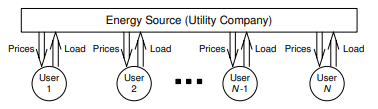
\includegraphics[width=0.75\textwidth]{img/teoria/dsm1.png}
  \caption{Estrategia de \gls{dsm} basada en interacciones individuales de cada consumidor con la compañía \cite{pricing}}
  \label{fig:dsm1}
\end{figure}

\vspace{3mm}

No obstante, el diseño de un programa \gls{dsm} ideal en el contexto de las \gls{sg}s debe permitir las interacciones entre los mismos usuarios dentro de una zona residencial o microgrid. Estas interacciones generalmente son automatizadas a través de una comunicación digital bidireccional. Como se aprecia en la Figura \ref{fig:dsm2}, este proceso tiene como fin conducir a una coordinación de las acciones respectivas a las cargas de un área determinada. 

\vspace{3mm}

\begin{figure}[h]
  \centering
  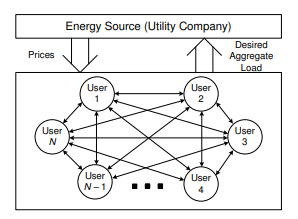
\includegraphics[width=0.6\textwidth]{img/teoria/dsm2.png}
  \caption{Estrategia de \gls{dsm} para smart grids basada en interacciones entre los usuarios y la compañía \cite{pricing}}
  \label{fig:dsm2}
\end{figure}

\vspace{3mm}

Por tanto, en este caso la monitorización de las cargas totales para todos los nodos participantes en un instante determinado aportará la información necesaria sobre la relación entre la potencia pico y promedio (del inglés \gls{par}) y contribuirá a la fijación del precio unitario para ese mismo instante. \cite{pricing} 


%%%%
 
%aqui hablar sobre fijación de precios towards concise models
\cite{towards}



\vspace{3mm}



%aqui hablar de ml para eficiencia de consumo



















\subsection{Protocolos}
%Green-RPL, Local positive degree coupling, IEEE 802.11s, Web Of Energy, Dynamic Barrier Coverage, IEC61850, Wind-driven bacterial foraging algorithm, Data Slicing, TSUBE energy trading algorithm, Stochastic Geometry, Rectangular quadrature amplitude modulation, Policy-based group authentication algorithm, Mapping interface integration COIIoT, Nash Equilibrium (NE) and the Bayesian NE, Wireless sensor network protocol and Algorithmic Approac

%ver tabla https://electrical-engineering-portal.com/smart-grid-deployment-what-weve-done-so-far




\subsection{Topología de red}
%NAN, FAN AND THE SDN are widely used network topology



\subsection{Tecnologías}
%Blockchain, Reinforcement Learning, Internet of Things, Machine learning, Data mining, Machine learning and neural training, Shortterm memory network, Power Line Communication Technology, Power electronics, Big data, Fog Cloudcomputing, Energy Storage, and Power Electronics Technologies










\subsection{Seguridad en Smart grids}

%ataques, tipos de ataques, como combatirlos
%a partir del 3.4 del AI-based FDI Countermeasure for IoE Smart Grids



%estándares smart grids -> cite OUTLOOK FOR INCREASED ADOPTION OF SMART GRID TECHNOLOGIES IN ADB ENERGY SECTOR OPERATIONS

% International Technical Standards for Smart Grids (Smart Grid Codes)
% Grid code development and implementation is a critical area in smart grid implementation. It has to be 
% aligned with the standards being used in respective countries and international standards. This is an 
% important first step in smart grid implementation. Some of the international standards are as follows.
% (i) IEEE1547 Family of Standards. IEEE 1547 family of standards deals with smart grid components 
% involving distributed resources interconnection. Released in 2003, this provides the basis and 
% sets the standards for the integration of distributed energy generation by detailing requirements 
% related to interconnection performance, operation, testing, safety, and maintenance.
% (ii) IEEE 2030 Family of Standards. The  IEEE Standard 2030–2011’s “Guide for Smart Grid 
% Interoperability of Energy Technology and Information Technology Operation with the 
% Electric Power System, and End-Use Applications and Loads” is the root standard of the 2030 
% series. This standard provides alternative approaches and best practices for achieving smart 
% grid interoperability.
% (iii) IEC Family of Standards. IEC has identified over 100 standards relevant to smart grids. The 
% following are core standards: (i) IEC/TR 62357: Service Oriented Architecture; (ii) IEC/61970: 
% Common Information Model/Energy Management; (iii) IEC 61850: Power Utility Automation; 
% (iv) ICC/61968: Common Information Model/Distribution Management; IEC 62351: Security; 
% (v) IEC 62056: Data Exchange for Meter Reading, Tariff and Load Control; and (vi) IEC 61508: 
% Functional Safety of Electrical, Electronic, Programmable Electronic Safety Related Systems.